\subsection{Direct Solver}
In this section we show the main results obtained with the implemented direct solver and we compare them with the ones from the out-of-the-box solver from \texttt{Numpy} library. As we show in the following paragraphs, our solver is able to achieve the expected precision and the achieved results are comparable with the ones obtained with the \texttt{Numpy} ones. However, we can't compare our solver to the \texttt{Numpy} one under an execution efficiency standpoint, since our solver lacks all the necessary optimizations needed to achieve the same performances as the library we used to compare our model with.

\subsubsection{QR implementation comparison}
In this section we show the comparison between the implemented algorithm \textbf{(A3)}, needed as an intermediate step for the \textit{LS} solution as specified in \S\ref{sec:qr}, and the \texttt{Numpy} out-of-the-box solver for the \textit{QR} computation.

\begin{figure}[H]
	\centering
	\begin{subfigure}{.45\textwidth}
	    \centering
	    \subcaptionbox{\label{img:a3_qr}}{%
            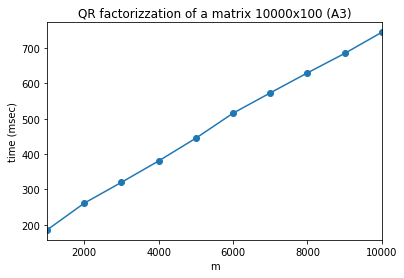
\includegraphics[width=\linewidth]{res/a3_scaling.png}\hspace*{1.5em}%
        }
	\end{subfigure}
	\begin{subfigure}{.45\textwidth}
	    \centering
	    \subcaptionbox{\label{img:np_qr}}{%
            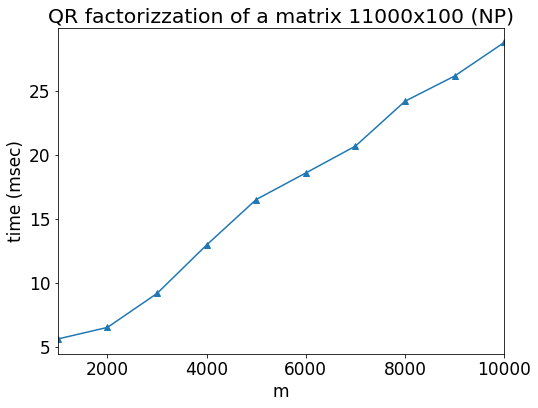
\includegraphics[width=\linewidth]{res/np_scaling.png}\hspace*{1.5em}%
        }
	\end{subfigure}
	
	\begin{subfigure}{.45\textwidth}
	    \centering
	    \subcaptionbox{\label{img:scaling}}{%
            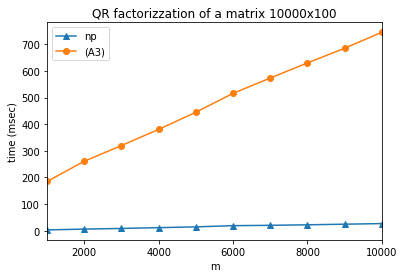
\includegraphics[width=\linewidth]{res/scaling_comp.png}\hspace*{1.5em}%
        }
	\end{subfigure}
    
	\caption{Comparison between the implemented \textbf{(A3)} algorithm with the \texttt{Numpy} off-the-shelf-solver. In figure \textbf{\ref{img:a3_qr}} and \textbf{\ref{img:np_qr}} there are, respectively, the performances in QR computation for the implemented \textbf{(A3)} solver and the \texttt{Numpy} one over datasets with increasing dimensions, up to 10000x100. In \textbf{\ref{img:scaling}} the same plots are put together to highlight the difference in performance.}
	\label{fig:scaling_qr}
\end{figure}

\vspace*{-1cm}
\begin{table}[H]
    \begin{center}
    \begin{adjustwidth}{0.cm}{}
    \begin{center}
    \resizebox{0.65\textwidth}{!}{%
    \begin{tabular}{|P{2.cm}||c|c|c|c|}
        \hline
         \textbf{m} & \textbf{time (A3)} & \textbf{delta (A3)} & \textbf{time (NP)} & \textbf{delta (NP)}\\ [0.5ex]
         \hline\hline
        1000 & 185.1129 & - & 3.1858 & -\\\hline
        2000 & 260.9890 & 75.8761 & 6.3108 & 3.1250\\\hline
        3000 & 319.9584 & 58.9694 & 8.6793 & 2.3686\\\hline
        4000 & 380.6262 & 60.6678 & 11.6935 & 3.0141\\\hline
        5000 & 444.9249 & 64.2987 & 14.6366 & 2.9432\\\hline
        6000 & 515.8109 & 70.8860 & 19.1323 & 4.4956\\\hline
        7000 & 573.2926 & 57.4817 & 20.4345 & 1.3022\\\hline
        8000 & 630.0169 & 56.7243 & 22.3729 & 1.9384\\\hline
        9000 & 685.0543 & 55.0375 & 24.7365 & 2.3636\\\hline
        10000 & 745.0878 & 60.0335 & 26.9332 & 2.1967\\\hline
    \end{tabular}}
    \end{center}
    \end{adjustwidth}
    \caption{Scaling performances of the implemented algorithm \textbf{(A3)} and the \texttt{Numpy} one. Time is expressed in milliseconds.}
    \label{tab:scaling_perf_qr}
    \end{center}
\end{table}
As we can see in both \hyperref[fig:scaling_qr]{\textbf{Figure \ref{fig:scaling_qr}}} and \hyperref[tab:scaling_perf]{\textbf{Table \ref{tab:scaling_perf_qr}}}, the implemented algorithm for \textit{QR} computation scales linearly with the \textbf{m} dimension of the matrix, as expected theoretically and as shown at the end of  \textbf{\S\ref{sec:ls_scaling}} paragraph. However, given that our algorithm does not make use of extensive optimizations, this reflects on the completion time required for the computation of the \textit{QR} factorization.

\subsubsection{LS implementation comparison}
In this paragraph we show the comparison between the implemented algorithm \textbf{(A3)} and the \texttt{Numpy} solver. We used a sequence of randomly generated matrix with increasing dimension \textit{m} in [1000, 10000], in order to highlight the scaling performances and show that they are in line with the theoretically expected ones. We decided to fix the \textit{n} dimension to 100 in order to allow the algorithm to terminate in a reasonable amount of time one the machine at our disposal.

\begin{figure}[H]
	\centering
	\begin{subfigure}{.4\textwidth}
	    \centering
	    \subcaptionbox{\label{img:a3_qr}}{%
            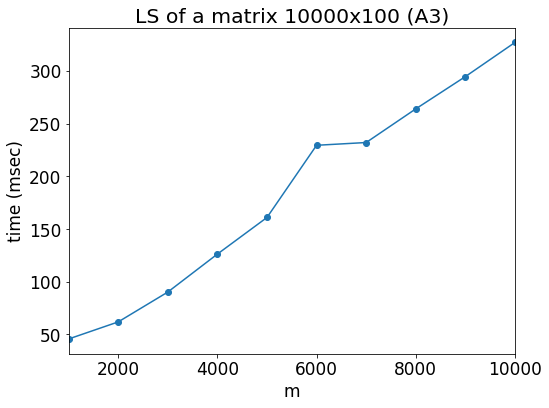
\includegraphics[width=\linewidth]{res/a3_ls_scaling.png}\hspace*{1.5em}%
        }
	\end{subfigure}
	\begin{subfigure}{.4\textwidth}
	    \centering
	    \subcaptionbox{\label{img:np_qr}}{%
            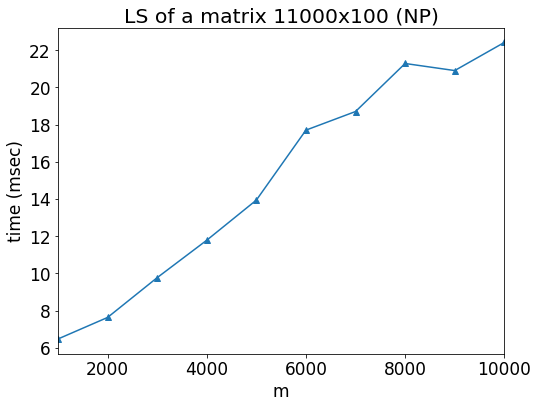
\includegraphics[width=\linewidth]{res/np_ls_scaling.png}\hspace*{1.5em}%
        }
	\end{subfigure}
	
	\begin{subfigure}{.4\textwidth}
	    \centering
	    \subcaptionbox{\label{img:scaling}}{%
            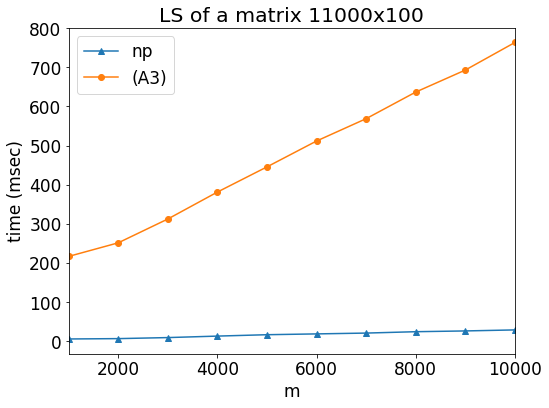
\includegraphics[width=\linewidth]{res/ls_scaling_comp.png}\hspace*{1.5em}%
        }
	\end{subfigure}
    
	\caption{Comparison between the implemented \textbf{(A3)} algorithm with the \texttt{Numpy} off-the-shelf-solver. In figure \textbf{\ref{img:a3_qr}} and \textbf{\ref{img:np_qr}} there are, respectively, the performances in LS computation for the implemented \textbf{(A3)} solver and the \texttt{Numpy} one. In \textbf{\ref{img:scaling}} the same plots are put together to highlight the difference in performance.}
	\label{fig:scaling_ls}
\end{figure}

\begin{table}[H]
    \begin{center}
    \begin{adjustwidth}{0.cm}{}
    \begin{center}
    \begin{tabular}{|P{2.cm}||c|c|c|c|}
        \hline
         \textbf{m} & \textbf{time (A3)} & \textbf{delta (A3)} & \textbf{time (NP)} & \textbf{delta (NP)}\\ [0.5ex]
         \hline\hline
        1000 & 33.2898 & - &    5.4329 & -\\\hline
        2000 & 61.8065 & 28.5167 & 8.0054 & 2.5725\\\hline
        3000 & 98.6733 & 36.8669 & 10.0943 & 2.0889\\\hline
        4000 & 128.8937 & 30.2204 & 11.8025 & 1.7082\\\hline
        5000 & 165.1421 & 36.2484 & 14.2208 & 2.4183\\\hline
        6000 & 208.6527 & 43.5106 & 16.6491 & 2.4283\\\hline
        7000 & 235.6089 & 26.9562 & 18.2518 & 1.6028\\\hline
        8000 & 275.4459 & 39.8371 & 20.8711 & 2.6193\\\hline
        9000 & 310.8279 & 35.3820 & 21.2367 & 0.3656\\\hline
        10000 & 334.9303  & 24.1024 & 22.9452 & 1.7085\\\hline
    \end{tabular}
    \end{center}
    \end{adjustwidth}
    \caption{Scaling performances of the implemented algorithm \textbf{(A3)} and the \texttt{Numpy} one. Time is expressed in milliseconds.}
    \label{tab:scaling_perf_ls}
    \end{center}
\end{table}

We can clearly see, both in \hyperref[fig:scaling_ls]{\textbf{Figure \ref{fig:scaling_ls}}} and \hyperref[tab_scaling_perf_ls]{\textbf{Table \ref{tab:scaling_perf_ls}}}, that the algorithm linearly scale with the \textit{m} dimension, as expected. Once again, the comparison under a computational efficiency standpoint can't be done properly, since our algorithm requires 10 times more with respect to the \texttt{Numpy} one.

Finally, in table \hyperref[tab:cup_res_direct]{\textbf{Table \ref{tab:cup_res_direct}}} we can see the results comparison in the Least Square solution for the CUP dataset by using the implemented solver and the one offered by the \texttt{Numpy} library. We also show the error in the reconstruction of the original matrix via \textit{QR} factorization and we can clearly see the goodness of the implementation with reference to highly optimized solvers.

\begin{table}[H]
    \begin{center}
    \begin{adjustwidth}{-0.4cm}{}
    \begin{center}
    \begin{tabular}{|P{2.cm}||c|c|c|c|}
        \hline
         \textbf{Task} & \textbf{residual (A3)} & \textbf{residual (NP)} & \textbf{QR to A (A3)} & \textbf{QR to A (NP)}\\ [0.5ex]
         \hline\hline
        CUP & 1.0538 & 0.9963 &  4.93339e-16 & 3.28932e-16\\
        \hline
        RANDOM & 1.0047 & 0.9953 & 7.89014e-16 & 3.92280e-16\\
        \hline
    \end{tabular}
    \end{center}
    \end{adjustwidth}
    \caption{Residual and reconstruction relative errors for the \textbf{(A3)} algorithm and the \texttt{Numpy} one.}
    \label{tab:cup_res_direct}
    \end{center}
\end{table}

However, even if the reconstruction error is up to machine precision, we can't state the same for what concerns the residual error for both of the compared algorithms. Since the problems are far from being linear, the solution found by the LS solver we used is very poor and it is close to the one achieved on a random dataset generated with a gaussian distribution.

As a final test, we checked if the precision in the results was maintaining at a stable and reasonable level also for bigger matrices. In \hyperref[tab:scaling_huge]{\textbf{Table \ref{tab:scaling_huge}}} we show the relative errors of the residual and the reconstruction error for datasets with the \textit{m} dimension in [10000, 50000] with scaling factor of 10000 while keeping the \textit{n} dimension once again fixed to 100.

\begin{table}[H]
    \begin{center}
    \begin{adjustwidth}{0.cm}{}
    \begin{center}
    \begin{tabular}{|P{2.cm}||c|c|c|c|}
        \hline
         \textbf{m} & \textbf{residual (A3)} & \textbf{residual (NP)} & \textbf{QR to A (A3)} & \textbf{QR to A (NP)}\\ [0.5ex]
         \hline\hline
        10000 & 1.004136 & 0.995936 & 1.148071e-15 & 5.144102e-16\\\hline
        20000 & 1.001552 & 0.997711 & 7.093753e-16 & 5.028219e-16\\\hline
        30000 & 1.001714 & 0.998399 & 6.781397e-16 & 4.979521e-16\\\hline
        40000 & 1.001585 & 0.998724 & 7.984209e-16 & 4.945500e-16\\\hline
        50000 & 1.001005 & 0.999045 & 8.001721e-16 & 4.950132e-16\\\hline
    \end{tabular}
    \end{center}
    \end{adjustwidth}
    \caption{Scaling performances of the implemented algorithm \textbf{(A3)} and the \texttt{Numpy} one.}
    \label{tab:scaling_huge}
    \end{center}
\end{table}

As we can see, also for this kind of test, the implemented algorithm attains a similar precision to the one provided by the \texttt{Numpy} library.